\chapter{Results and discussion}

In this chapter we present the results of \gls*{db} characterization in two measured proteins, and one in-silico generated dataset. We also provide some supporting data justifying our choice of scoring metric and the design of the matching algorithms. Finally, we evaluate the results, concluding that many \glspl*{db} are successfully identified, although there are many false positive fragment matches.

\section{Dibby scores correctly reflect false positive fragment assignments}

In the proteins we analysed, the theoretical positions of \glspl*{db} are known. We call a fragment (and by extension, the whole variant) that contradicts the knowledge about \gls*{db} positions a \emph{bad} fragment. We have evaluated our variant scoring metric on four different datasets (\gls*{lys}, \gls*{lip}, \gls*{genova}, and \gls*{bsa}), separately on good and bad variants; the results are shown on \Cref{fig:scoring-metric}. A clear difference between the median variant score of the bad and the good variants can be seen.

\begin{figure}
  \centering
  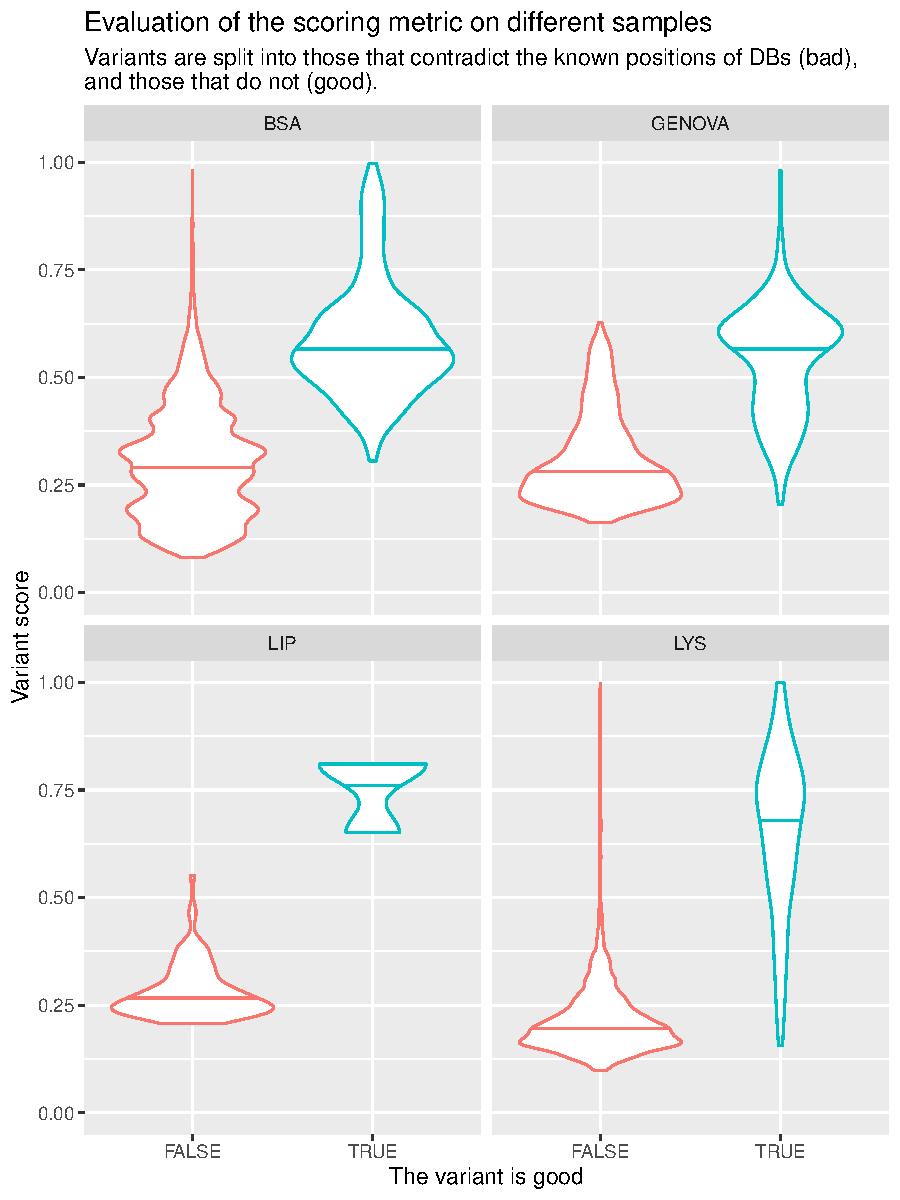
\includegraphics[width=0.85\linewidth]{img/scoring-metric-evaluation.pdf}
  \caption{Scoring metric evaluation on datasets from four different samples. Individual data points represent different assigned variants, that are grouped based on whether they contradict expert knowledge about \gls*{db} positions. The box plots illustrate that the separation is usually relatively good, but as we can see from the data points, there are still a lot of (in theory) non-existent variants with a high score. This can partly be attributed to \gls*{db} scrambling. The lack of data in the \gls*{lip} sample is discussed in the text. (\gls*{bsa} = bovine serum albumin, \gls*{lys} = lysozyme, \gls*{lip} = lipase, \gls*{genova} = an in-silico generated ovalbumin dataset)}\label{fig:scoring-metric}
\end{figure}

\section{Dibby identifies existing \glspl*{db}}

A complete \gls*{db} analysis has been performed on three proteins, namely \gls*{lys}, \gls*{lip}, and \gls*{genova}\@. The analysis was initially run with vanilla settings. If there had been a strong evidence for a particular \gls*{db} in the RAT data, it was deemed to be prone to generating false positive signals. Consequently, its weight has been adjusted to 0.1, or 0.8, depending on the strength of its RAT evidence, and the analysis was run again.

The results from the second run of the analysis can be seen on the following figures: \Cref{fig:lys} (\gls*{lys}), \Cref{fig:lip} (\gls*{lip}), and \Cref{fig:genova} (\gls*{genova}). The top row shows data from RAT samples, the bottom shows data from AT samples, the left column shows the theoretical positions of the cysteine alkylations and disulphide bonds, and the right column shows the aggregated evidence. Alkylation evidence is illustrated by a border around the cysteine.

As is apparent from the images, Dibby generates a lot of false positive signal. However, the scoring and weighting of the evidence helps immensely, and some \glspl*{db} are still clearly identifiable; three in the \gls*{lys} sample (of the four total \glspl*{db}), one in the \gls*{lip} sample (of the three total \glspl*{db}), and one in the \gls*{genova} sample (the only \gls*{db} that is present).


\paragraph{Lysozyme} Three of the four \glspl*{db} have been identified (\Cref{fig:lys}). The evidence for the last \gls*{db} has been seen in only 7 good fragments, compared for example to the 2,534 good fragments of the bond \((5, 126)\). We are not sure what caused this stark disparity, and the causes should be more deeply investigated in the future. The evidence for the bond \((75, 93)\) is not as strong as for the other two, relative to the evidence for alkylations of the respective cysteines. \((75, 93)\) is objectively hard to identify, because there is no tryptic cleavage point between the cysteines. The fact that Dibby has been able to identify this bond foreshadows the power of its general assignment algorithm.

\begin{figure}
  \centering
  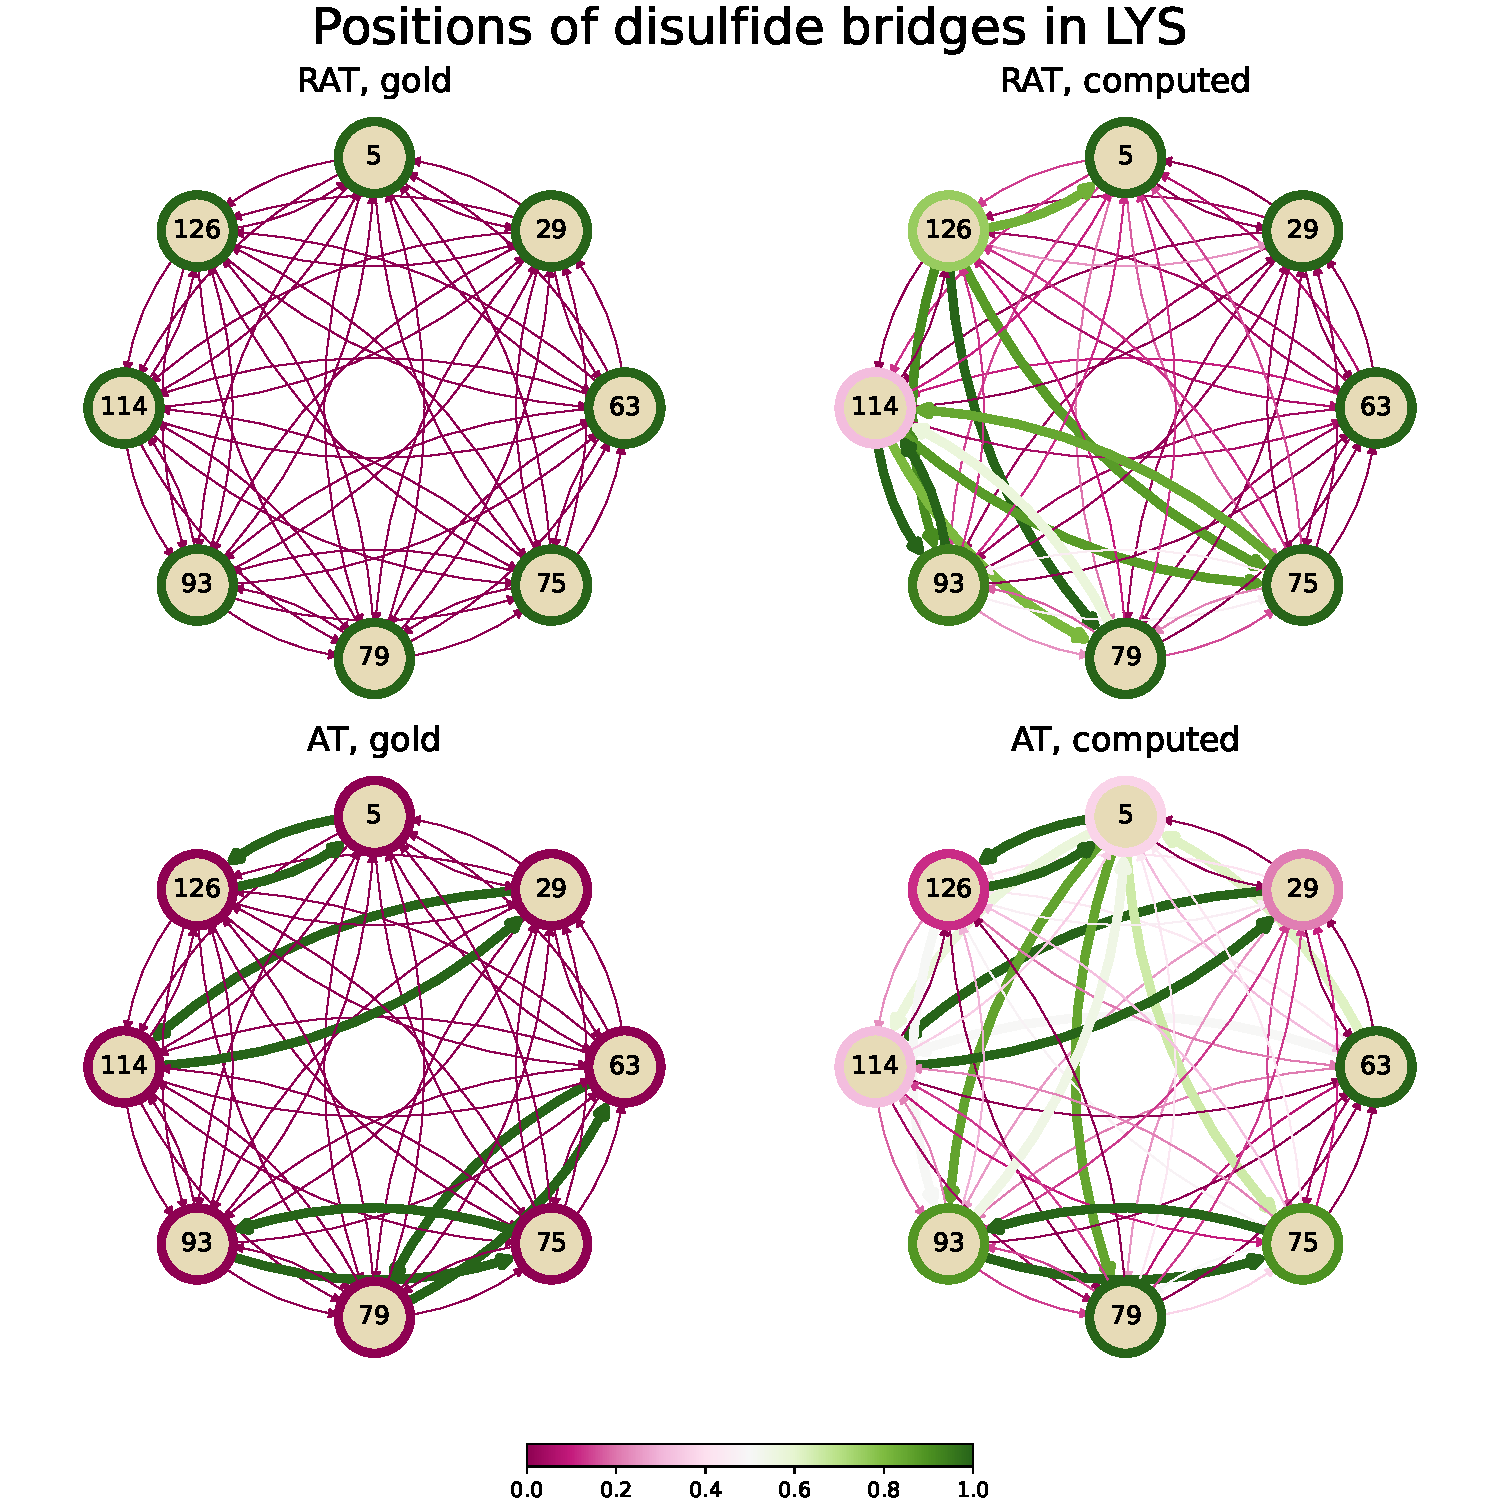
\includegraphics[width=0.9\linewidth]{img/lys.pdf}
  \caption{The evidence for positions of \glspl*{db} and alkylations in lysozyme, weighted by variant score, and normalized. There are quite a few false positives, however, the bonds \((5, 126)\) and \((29, 114)\) are still clearly visible. We can safely ignore the other directed edges stemming from 5, because their scores are relatively low compared to \((5, 126)\), and also because they are not bidirectional --- that means that the supposed bond-partners are seen more commonly in other configurations. The presence of the bond \((75, 93)\) is not so clear-cut; we also have strong signals about the cysteines being alkylated. This warrants further investigation. Finally, the evidence for bond \((63, 79)\) is practically not present, and both cysteines were deemed as alkylated.}\label{fig:lys}
\end{figure}

\paragraph{Generated ovalbumin} Similarly to the lysozyme plots, some false positives had cropped up (\Cref{fig:lip}), though they did not manage to drown out the true evidence. The only present \gls*{db}, \((72, 119)\), has been successfully identified. There are some directed edges coming into the cysteine 119, however; the algorithm and the scoring system should be fine-tuned so that similar false positives do not slip through the cracks, or at least do not provide such a strong signal.

\begin{figure}
  \centering
  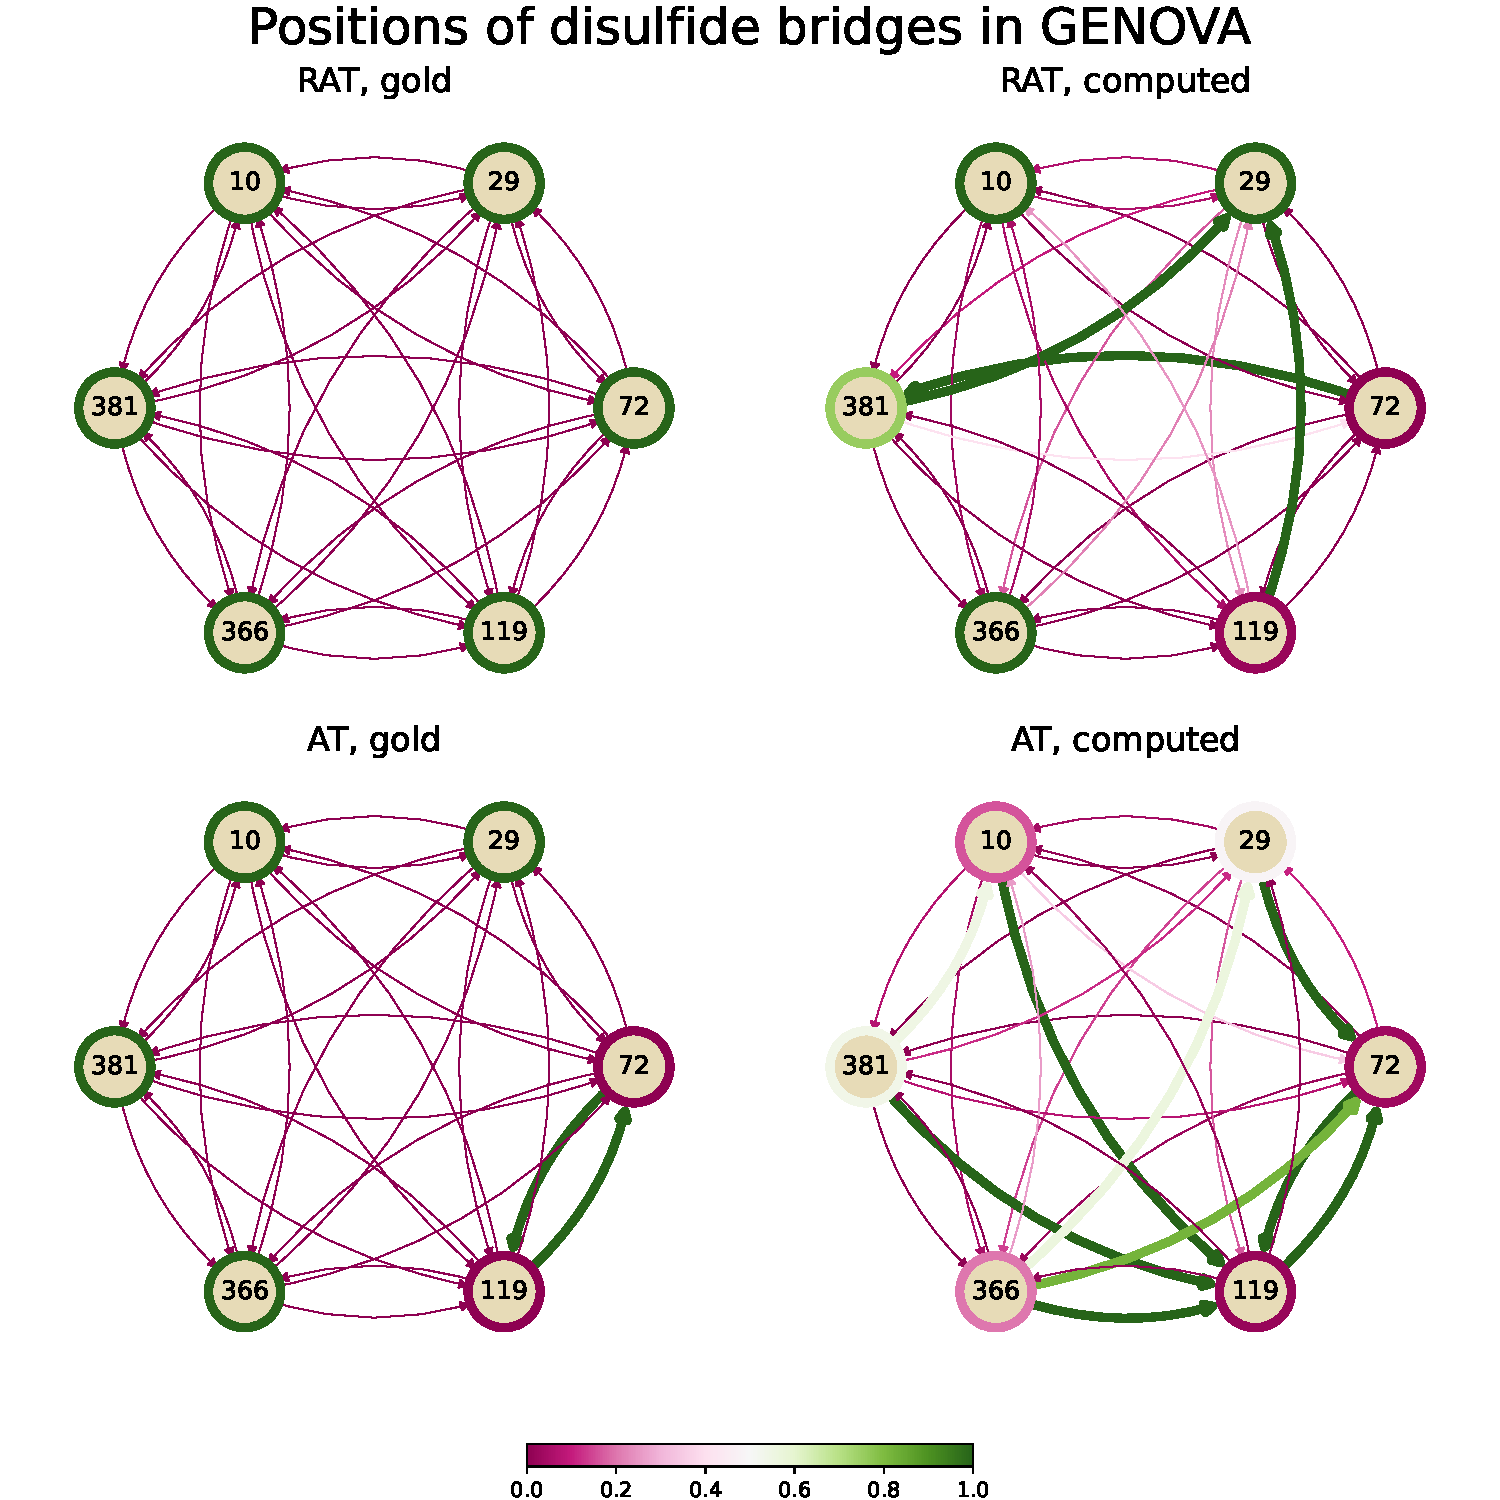
\includegraphics[width=0.9\linewidth]{img/genova.pdf}
  \caption{The evidence for positions of \glspl*{db} and alkylations in in-silico generated ovalbumin, weighted by variant score, and normalized. Although there are some false positives, the only confirmed bidirectional bond is also the correct one: \((72, 119)\).}\label{fig:genova}
\end{figure}

\paragraph{Lipase} Only one of the three \glspl*{db} has been identified in the \gls*{lip} sample (\Cref{fig:lip}). Interestingly, we have identified exactly zero variants containing the cysteines 271 and 295, alkylated or otherwise. To test whether this had been caused by a problem in the data or the algorithm, we have run a MSGF+~\cite{kim2014ms} analysis on the \gls*{lip} samples (and later on the other samples as well); the comparison with results from Dibby is in \Cref{tbl:measurements}. We can see that even MSGF+, a state of the art proteomic database search tool, had problems with \gls*{lip} data, suggesting an unknown issue occurred during the sample preparation, rendering most of the \gls*{lip} data unusable.

\begin{table}[ht]
  \begin{tabular}{@{}llllll@{}}
    \toprule
    \multicolumn{1}{c}{\multirow{2}{*}[-0.25em]{Sample}} & \multirow{2}{*}[-0.25em]{Scans} & \multicolumn{1}{c}{\multirow{2}{*}[-0.2em]{\begin{tabular}[c]{@{}c@{}}MSGF+\\ Matches\end{tabular}}} & \multicolumn{3}{c}{Dibby matches}                       \\ \cmidrule(l){4-6}
    \multicolumn{1}{c}{}                                 &                                 & \multicolumn{1}{c}{}                                                   & Simple                            & Total & \glspl*{db} \\ \midrule
    \gls*{lys} AT                                        & 12479                           & 411                                                                    & 463                               & 2240  & 3/4         \\
    \gls*{lys} RAT                                       & 14517                           & 1216                                                                   & 2157                              & 2972  &             \\
    \gls*{lip} AT                                        & 13579                           & 21                                                                     & 12                                & 67    & 1/3         \\
    \gls*{lip} RAT                                       & 14177                           & 76                                                                     & 66                                & 131   &             \\
    \gls*{genova} AT                                     & 1606                            &                                                                        & 855                               & 3257  & 1/1         \\
    \gls*{genova} RAT                                    & 735                             &                                                                        & 770                               & 805   &             \\
    \gls*{bsa} AT                                        & 13856                           & 1495                                                                   & 1717                              & 48222 &             \\
    \gls*{bsa} RAT                                       & 14242                           & 1723                                                                   & 2684                              & 22133 &             \\ \bottomrule
  \end{tabular}
  \caption{Comparison of Dibby with MSGF+, a state-of-the-art database search tool for proteomics. MSGF+ can only identify peptides that are not cross-linked, or ``simple'' peptides; for this reason, we list the number of Dibby's simple assignments in addition to the total number of its assignments. Generally, Dibby identifies a bit more simple precursors than MSGF+, most of which are probably false positives. On the other hand, there are close to 0 false negatives. There is clearly a problem with lipase data; MSGF+ identified 16 times more precursors in the \gls*{lys} RAT sample than in \gls*{lip} RAT, although the number of measured scans in the mgf file is comparable between these two samples.}\label{tbl:measurements}
\end{table}

\begin{figure}
  \centering
  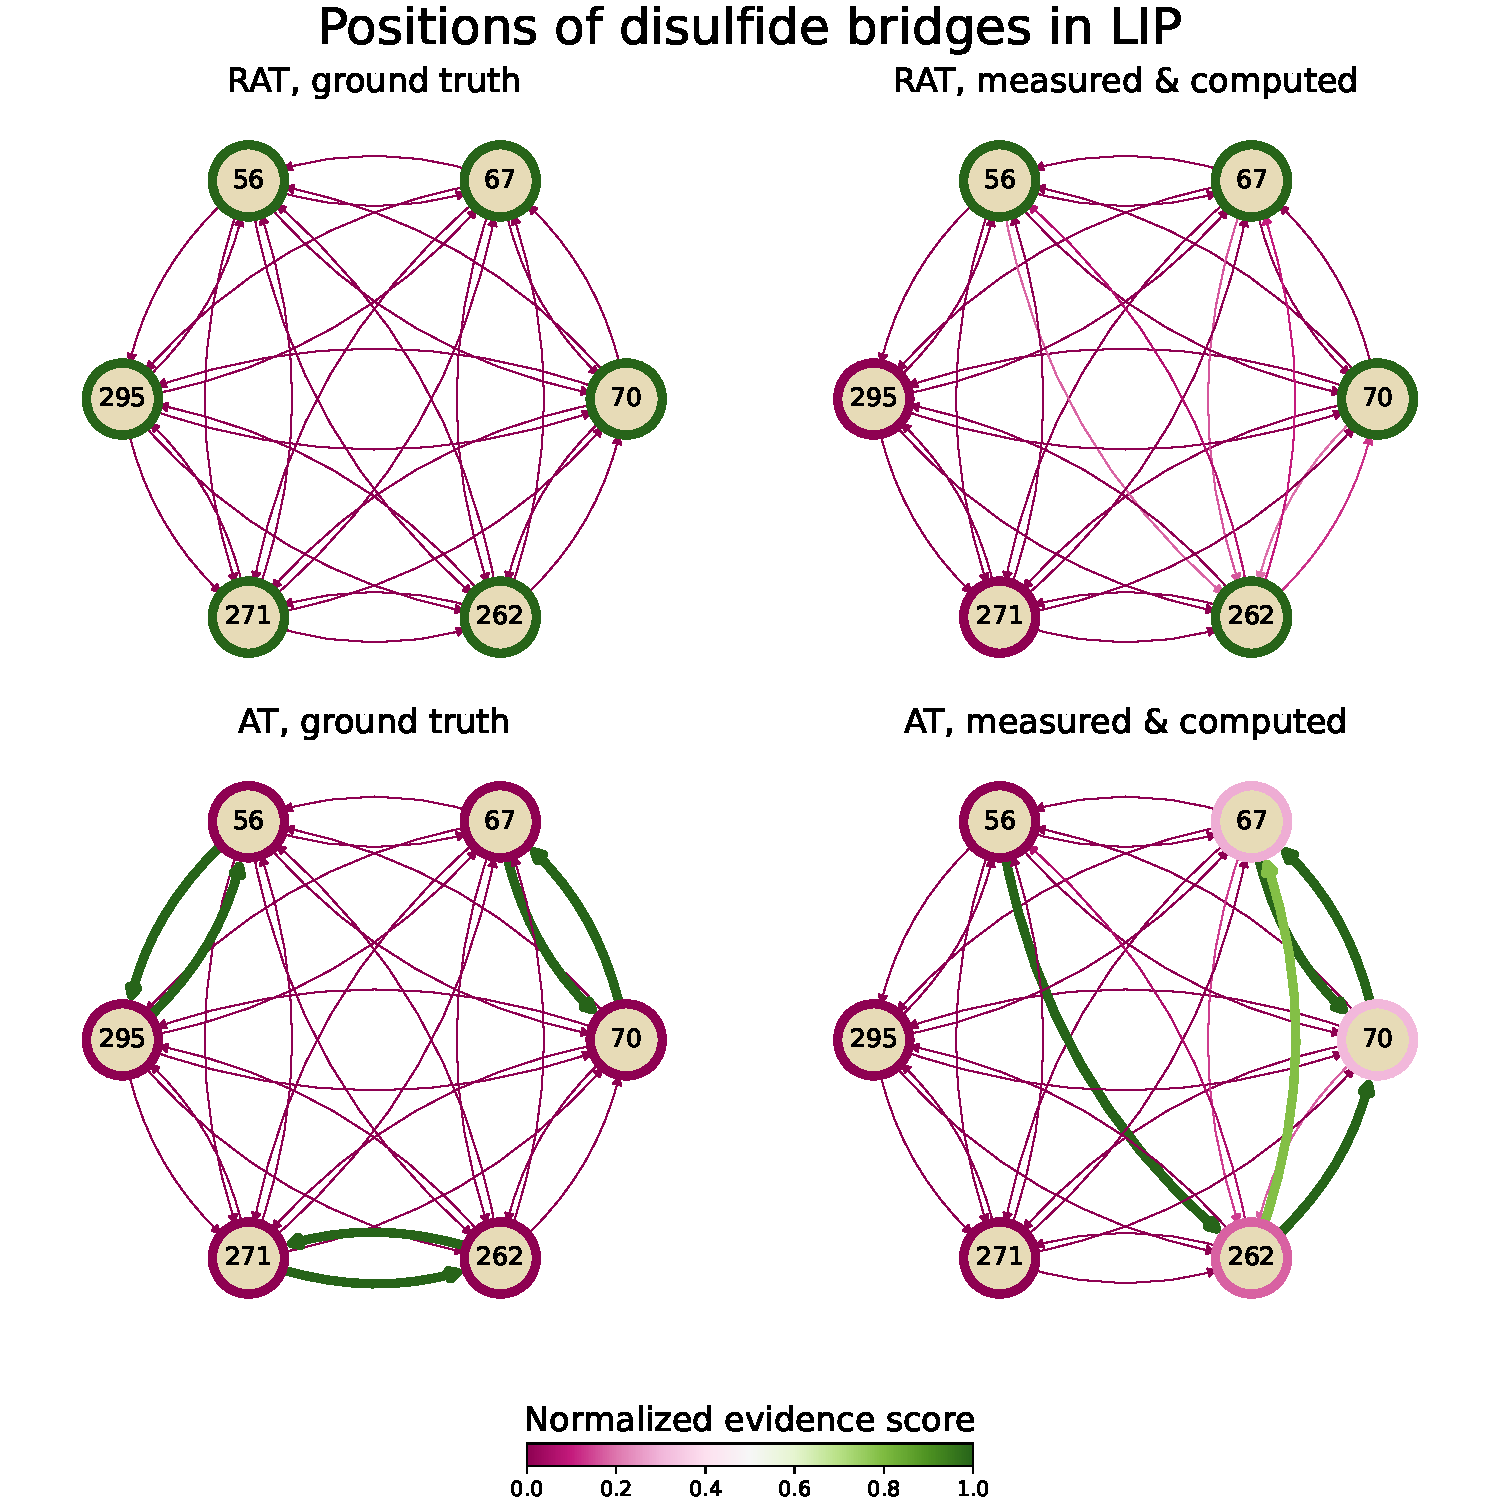
\includegraphics[width=0.9\linewidth]{img/lip.pdf}
  \caption{The evidence for positions of \glspl*{db} and alkylations in in-silico generated ovalbumin, weighted by variant score, and normalized. No fragments containing cysteines 271 and 295 have been assigned (neither in alkylated form, nor as a part of any disulphide bond); this leads us to believe that a part of the data has been lost, or otherwise damaged.}\label{fig:lip}
\end{figure}

To conclude, the scoring metric separates good variants from the bad ones rather well. With the help of the scoring system, Dibby managed to sift through the large number of false positive fragment assignments, and successfully identified most of the true \glspl*{db} in the \gls*{lys} and \gls*{genova} samples. One true \gls*{db} has even been identified in \gls*{lip}, despite the problems in the \gls*{lip} dataset.


\section{Discussion}

In the discussion below, we do not consider the results obtained from the \gls*{lip} samples, because --- as we have shown --- there has been an unknown issue during the measurements, rendering the data unreliable.

\paragraph{Scoring} In order for the scoring metric to be useful, bad fragments and variants should generally have a lower score than good ones, presuming the measured data correlates with the expert knowledge about \gls*{db} positions. We have indeed found that the metric satisfactorily separates the good variants from the bad ones (see \Cref{fig:scoring-metric}), nonetheless there are still many bad variants with a high score, especially in the \gls*{bsa} and \gls*{lys} datasets. A possible explanation is that although \glspl*{db} that contradict expert knowledge should not be present in the data \emph{in theory}, due to \gls*{db} scrambling they \emph{are} present; subsequently, variants containing these bonds receive a high score because they match the measured data well, but are labelled as bad during our evaluation of the scoring metric (\Cref{fig:scoring-metric}). This hypothesis is further supported by the absence of the high-scoring bad variants from the generated \gls*{genova} dataset, in which no \gls*{db} scrambling has occurred.

\paragraph{\gls*{db} characterization} Despite the strong signal from false positive matches, and the complications resulting from \gls*{db} scrambling, most of the \glspl*{db} present in \gls*{lys} (\Cref{fig:lys}) and \gls*{genova} (\Cref{fig:genova}) have been identified. Especially important is the \gls*{lys} \gls*{db} \((75, 93)\), an intra-peptide \gls*{db} that would be hard to identify with other methods. This demonstrates the flexibility and raw matching power of the algorithm. However, more work needs to be done to lower the false discovery rate. After improvements in this area, and potentially some changes to the data preparation protocol, Dibby could be used to assist researchers with \gls*{db} mapping in proteins.

\paragraph{Manual analysis} In addition to the visualizations, a csv file with the fragment assignments is generated by Dibby. This enables researchers to perform detailed manual analysis based on data from Dibby's matching algorithms, or to manually check the evidence for a specific \gls*{db} to verify the results. In the future, the match data could be used to perform automatic labelling of matched fragments, including complex internal fragments with multiple modifications and disulphide bonds, a task that is as of now still not solvable by any tool.

In conclusion, Dibby has managed to identify most \glspl*{db} from the analysed dataset, including one intra-peptide bond. We have also shown the importance of protease choice during the sample preparation phase by identifying variants that possibly resulted from \gls*{db} scrambling during tryptic digestion. Some of Dibby's pain points were highlighted, suggesting a topic for future research.
